%% file: template.tex = LaTeX template for article-like report 
%% init: sometime 1993
%% last: Oct  2 2016  Rob Rutten  Deil
%% site: http://www.staff.science.uu.nl/~rutte101/rrweb/rjr-edu/manuals/student-report/

%% First read ``latex-bibtex-simple-manual.txt'' at
%% http://www.staff.science.uu.nl/~rutte101/Report_recipe.html

%% Start your report production by copying this file into your XXXX.tex.
%% Small changes to the header part will make it an A&A or ApJ manuscript.

%%%%%%%%%%%%%%%%%%%%%%%%%%%%%%%%%%%%%%%%%%%%%%%%%%%%%%%%%%%%%%%%%%%%%%%%%%%%
\documentclass{aa-note}   %% Astronomy & Astrophysics style class v8.2

\usepackage{graphicx,natbib,url,twoopt}
\usepackage[varg]{txfonts}           %% A&A font choice
\usepackage{hyperref}                %% for pdflatex
%%\usepackage[breaklinks]{hyperref}  %% for latex+dvips
%%\usepackage{breakurl}              %% for latex+dvips
\usepackage{pdfcomment}              %% for popup acronym meanings
\usepackage{acronym}                 %% for popup acronym meanings

\hypersetup{
  colorlinks=true,   %% links colored instead of frames
  urlcolor=blue,     %% external hyperlinks
  linkcolor=red,     %% internal latex links (eg Fig)
  citecolor=blue,
}

\bibpunct{(}{)}{;}{a}{}{,}    %% natbib cite format used by A&A and ApJ

\pagestyle{plain}   %% undo the fancy A&A pagestyle 

%% Add commands to add a note or link to a reference
\makeatletter
\newcommand{\bibnote}[2]{\global\@namedef{#1note}{#2}}
\newcommand{\biblink}[2]{\global\@namedef{#1link}{#2}}
\makeatother

%% Commands to make citations ADS clickers and to add such also to refs
%% May 2014: they give error stops ("Illegal parameter number ..."}
%%   for plain latex with TeX Live 2013; the ad-hoc fixes added below let
%%   latex continue instead of stop within these commands.
%%   Please let me know if you know a better fix!
%%   No such problem when using pdflatex.
\makeatletter
 \newcommandtwoopt{\citeads}[3][][]{%
   \nonstopmode%              %% fix to not stop at error message in latex
   \href{http://adsabs.harvard.edu/abs/#3}%
        {\def\hyper@linkstart##1##2{}%
         \let\hyper@linkend\@empty\citealp[#1][#2]{#3}}%   %% Rutten, 2000
   \biblink{#3}{\href{http://adsabs.harvard.edu/abs/#3}{ADS}}%
   \errorstopmode}            %% fix to resume stopping at error messages 
 \newcommandtwoopt{\citepads}[3][][]{%
   \nonstopmode%              %% fix to not stop at error message in latex
   \href{http://adsabs.harvard.edu/abs/#3}%
        {\def\hyper@linkstart##1##2{}%
         \let\hyper@linkend\@empty\citep[#1][#2]{#3}}%     %% (Rutten 2000)
   \biblink{#3}{\href{http://adsabs.harvard.edu/abs/#3}{ADS}}%
   \errorstopmode}            %% fix to resume stopping at error messages
 \newcommandtwoopt{\citetads}[3][][]{%
   \nonstopmode%              %% fix to not stop at error message in latex
   \href{http://adsabs.harvard.edu/abs/#3}%
        {\def\hyper@linkstart##1##2{}%
         \let\hyper@linkend\@empty\citet[#1][#2]{#3}}%     %% Rutten (2000)
   \biblink{#3}{\href{http://adsabs.harvard.edu/abs/#3}{ADS}}%
   \errorstopmode}            %% fix to resume stopping at error messages 
 \newcommandtwoopt{\citeyearads}[3][][]{%
   \nonstopmode%              %% fix to not stop at error message in latex
   \href{http://adsabs.harvard.edu/abs/#3}%
        {\def\hyper@linkstart##1##2{}%
         \let\hyper@linkend\@empty\citeyear[#1][#2]{#3}}%  %% 2000
   \biblink{#3}{\href{http://adsabs.harvard.edu/abs/#3}{ADS}}%
   \errorstopmode}            %% fix to resume stopping at error messages 
\makeatother

%% ADS specific page opener = {bibcode}{pdf page number}{link text}
\def\linkadspage#1#2#3{\href{http://adsabs.harvard.edu/cgi-bin/nph-data_query?bibcode=#1\&link_type=ARTICLE\&d_key=AST\#page=#2}{#3}}

%% Acronyms
\newacro{ADS}{Astrophysics Data System}
\newacro{NLTE}{non-local thermodynamic equilibrium}
\newacro{NASA}{National Aeronautics and Space Administration}

%% Add popups with meaning to acronyms 
%% NB: only show up in Adobe Reader and do not work with \input or \include
\gdef\acp#1{%
  \pdfmarkupcomment[markup=Underline,color={1 1 1},author={{#1}},opacity=0]%
  {{#1}}{{\acl{#1}}}}

%% Spectral species
\def\MgI{\ion{Mg}{I}}          %% A&A; for aastex use \def\MgI{\ion{Mg}{1}} 
\def\MgII{\ion{Mg}{II}}        %% A&A; for aastex use \def\MgII{\ion{Mg}{2}} 

%% Hyphenation
\hyphenation{Schrij-ver}       %% Dutch ij is a single character

\usepackage{amssymb,bm}
\usepackage{array}

%%%%%%%%%%%%%%%%%%%%%%%%%%%%%%%%%%%%%%%%%%%%%%%%%%%%%%%%%%%%%%%%%%%%%%%%%%%%
\begin{document}  

%% simple header.  Change into A&A or ApJ commands for those journals

\twocolumn[{%
\vspace*{4ex}
\begin{center}
%  {\Large \bf Frequency-position relation of extragalactic sources from the ICRF3 and \textit{Gaia} DR2}\\[4ex]       
   {\Large \bf Comparison of multi-frequency positions of extragalactic sources}\\[4ex] 
  {\large \bf 
              Niu Liu$^{1}$, 
              S\'ebastien Lambert$^2$,
              Cheng-Yu Ding$^1$,
              Zi Zhu$^1$,
              and 
              Jia-Cheng Liu$^1$
          }\\[4ex]
  \begin{minipage}[t]{15cm}
        $^1$ School of Astronomy and Space Science,
   		     Key Laboratory of Modern Astronomy and Astrophysics (Ministry of Education), 
		     Nanjing University, Nanjing, P. R. China\\
        $^2$ SYRTE, Observatoire de Paris,
             Universit\'e PSL, CNRS, Sorbonne Universit\'e, LNE, Paris, France\\
%        $^3$ Institute3\\
			%\email{liuniu@smail.nju.edu.cn;zhuzi@nju.edu.cn}
            %\email{sebastien.lambert@obspm.fr}

  {\bf Abstract.}
  % Context  
  Previous comparisons of the \textit{Gaia} and radio positions measured by the very long baseline interferometry (VLBI) at $X$-band probes the structure of the milli-arcsecond (mas) scale of Active Galactic Nucleus.
  But the available VLBI positions at high frequencies are less tapped.
  % Aims
  We aim to study the multi-frequency position of extragalactic sources, complementary to previous studies
  % Methods
  We compared the absolute positions measured at four different bands, 
  that is, optical position from the {\it Gaia} Data Release 2,and three radio position at $X$-, $K$-, and $Ka$-band from the ICRF3 catalog for 488 common sources.
  We aligned the $K$-band, $Ka$-band, and \textit{Gaia}-CRF onto the $X$-band frame, and then calculated the radio-to-optical offsets.
  We compared the radio-to-optical offset measured at different bands and correlated them with the magnitude, source structure index, and morphological indices.
  % Results
  The absolute difference of radio-to-optical offsets at different radio bands is less than 0.2~mas for 91\% of the sample.
  The large radio-to-optical offset appears to favor faint quasars, while we did not detect obvious correlation on other parameters. 
  We found 57 sources with four-band positions aligned, among which more than half sources have a radio-to-optical offset parallel to their jet when the jet direction is available.
  However, this position-alignment relation is vulnerable to the global systematics.
  % Conclusion
  The source structure does not affect much the radio source position at $X$-band.
  The selection criteria of optically bright radio-loud sources for frame-link at $X$-band might also work for the $K$- and $Ka$-band.
  Our result justify the reliability of the ICRF3 $X$-band frame.
  \vspace*{2ex}
  \end{minipage}
\end{center}
}] 


%%%%%%%%%%%%%%%%%%%%%%%%%%%%%%%%%%%%%%%%%%%%%%%%%%%%%%%%%%%%%%%%%%%%%%%%%%%%
\section{Introduction}     \label{sec:introduction}
%%%%%%%%%%%%%%%%%%%%%%%%%%%%%%%%%%%%%%%%%%%%%%%%%%%%%%%%%%%%%%%%%%%%%%%%%%%%

The frequency-dependent position of extragalactic objects (mostly distant quasars) is of interest in both astrometric and astrophysical fields, especially the position offset between the optical centroid and radio core.
Such studies can be used to maintain and improve the celestial reference frames materialized by positions of extragalactic objects. 
For example, the optical observations of the ICRF2 sources in the Rio survey monitors the frame-link status between the \textit{Hipparcos} celestial reference frame and the International Celestial Reference Frame (ICRF) \citep{2013MNRAS.430.2797A}.
The study of radio-to-optical offset also provides a probing of the structure properties of Active Galactic Nucleus (AGN), such as the accretion disc and relativistic jet \citep[e.g.,][]{2019ApJ...871..143P}. 

Accurate positions at sub-milli-arcsecond (mas) are needed for studying the frequency-position relation, which was achieved exclusively by the  very long baseline interferometry (VLBI) in the past.
The arrival of \textit{Gaia} Data release 2 \citep[\textit{Gaia} DR2;][]{2016A&A...595A...1G,2018A&A...616A...1G} data provides optical positions of quasars with a precision close to their VLBI positions.
The comparison between \textit{Gaia} and VLBI positions measured at 8~GHz shows excellent agreements on the level of 1~mas except about 6-9 per cent of outliers, that is, significant \textit{Gaia}/VLBI offsets \citep{2016A&A...595A...5M,2018A&A...616A..14G,2017MNRAS.471.3775P,2017MNRAS.467L..71P,2017A&A...598L...1K,2017ApJ...835L..30M,2018AJ....155..229F,2019MNRAS.482.3023P,2019ApJ...871..143P,2020MNRAS.493L..54K}.
Recently, \citet{2019MNRAS.482.3023P} report that for 62\% of sources with a significant \textit{Gaia}/VLBI offset and determinable jet direction, the VLBI-to-\textit{Gaia} offset vector is parallel to the jet.
\citet{2019ApJ...871..143P,2020MNRAS.493L..54K} further extend this study and find a correlation between the \textit{Gaia}/VLBI offset parallel to jet direction with the dominance of host galaxy, accretion disc, and jet in the optical domain.

These studies, however, are only limited to the VLBI positions at $X$-band.
Note that VLBI positions at higher frequencies, such as $K$- and $Ka$-band, are also feasible, showing competing precisions to that of $X$-band \citep[e.g.,][]{2019evga.confP.302J,2019evga.confP.306D}.
The $K$- and $Ka$-band positions suffer less from the radio source structure and ionosphere and solar plasma effects than at $X$-band \citep[e.g.,][]{2002ivsg.conf..350J}.
Including $K$- and $Ka$-band positions in the \textit{Gaia}/VLBI offset studies would help understand the origin of the radio-to-optical offsets.
On the other side, the link between $K$- and $Ka$-band VLBI frames and the \textit{Gaia} celestial reference frame (\textit{Gaia}-CRF) also requires detailed studies on the position offsets between $K$- and $Ka$-band and \textit{Gaia}.

We aim to compare the multi-frequency positions of extragalactic sources, in order to complement findings led by \citet{2019MNRAS.482.3023P}.
We computed the \textit{Gaia}/VLBI offsets at $X$-, $K$-, and $Ka$-band and studied their dependency on the astrophysical parameters, such as the magnitude, redshift, source structure at radio and optical domain, in order to provide new insights to understanding of the origin of radio-to-optical, as well as improving the link between \textit{Gaia}-CRF and VLBI frames other than $X$-band.

%%%%%%%%%%%%%%%%%%%%%%%%%%%%%%%%%%%%%%%%%%%%%%%%%%%%%%%%%%%%%%%%%%%%%%%%%%%%
\section{Data and methods}    \label{sec:obs}
%%%%%%%%%%%%%%%%%%%%%%%%%%%%%%%%%%%%%%%%%%%%%%%%%%%%%%%%%%%%%%%%%%%%%%%%%%%%

We used the radio positions of quasars measured by VLBI at $X$-, $K$-, and $Ka$-band from the ICRF3 catalog publicly available at the Paris Observatory IERS ICRS Center\footnote{\url{http://hpiers.obspm.fr/icrs-pc/newwww/icrf/index.php}}.
For positions of their optical counterparts, we took the \textit{Gaia}-CRF2 sample (\texttt{gaiadr2.aux\_iers\_gdr2\_cross\_id} table) from the \textit{Gaia}-DR2 archive\footnote{\url{http://gea.esac.esa.int/archive/}}.
The cross-match amongst these four catalogs gave a list of 488 common sources.

The median formal uncertainties on the right ascension, declination, and along the semi-major axis of error ellipse are $\mathrm{43\,\mu as}$, $\mathrm{53\,\mu as}$, and $\mathrm{55\,\mu as}$, respectively, for the $X$-band positions.
The corresponding values are $\mathrm{66\,\mu as}$, $\mathrm{126\,\mu as}$, and $\mathrm{128\,\mu as}$ for their $K$-band positions; 
$\mathrm{67\,\mu as}$, $\mathrm{98\,\mu as}$, and $\mathrm{104\,\mu as}$ at $Ka$-band; 
and $\mathrm{189\,\mu as}$, $\mathrm{167\,\mu as}$, and $\mathrm{218\,\mu as}$ for \textit{Gaia} positions. 
Therefore, the $X$-band position precision is generally twice better than the $K$- and $Ka$-band, and nearly four times better than the \textit{Gaia} DR2 positions for the sample used here.

Even the ICRF3 and the \textit{Gaia}-CRF2 are both the realizations of the International Celestial Reference System \citep[ICRS;][]{1995A&A...303..604A,1998A&A...331L..33F}, \citet{2020A&A...634A..28L} have revealed some zonal (declination-dependent) errors as large as 0.2~mas in the $Ka$-band frame, which might bias our analyses here.
In order to model and, subsequently, remove these systematical differences, 
we used the vector spherical harmonics \citep[VSH;][]{2012A&A...547A..59M} of degree 2, whose equation could be found in \citet[][their Eq.~(1)]{2020A&A...634A..28L}.
We followed similar procedures described therein to determine 16 transformation parameters between celestial reference frames at different wavelengths, except that we did not perform any outlier elimination.
(The influence of outliers on our results are discussed in Sect.~\ref{subsec:sys-effect}.)
The $X$-band celestial frame was chosen as the reference frame since it is most accurate celestial reference frame so far.
By doing so, we permit to analyze multi-wavelength positions in a consist celestial frame and avoid possible bias arising from the alignment and deformation of the celestial reference frames.

We then measured three radio-to-optical offsets, that is, the angular separation between $X$-, $K$-, and $Ka$-band and \textit{Gaia} positions.
We also computed the normalized separation, that is, the $X$-statistics given in the \citet{2016A&A...595A...5M}, 
to account for the formal uncertainty and correlation between right ascension and declination of individual sources.
These two quantities serve as indicators of significant radio-to-optical offset as done in recent works \citep[e.g.,][]{2019MNRAS.482.3023P,2018A&A...616A..14G}.

In order to study the correlation between radio-to-optical distances and astrophysical properties of the quasars, we used the $G$ magnitude given in the {\it Gaia} DR2 catalogs.
Besides, we collected the structure index \citep[SI;][]{1997ApJS..111...95F} at $X$-band from the Bordeaux VLBI Imaging database (BVID) \footnote{\url{http://bvid.astrophy.u-bordeaux.fr/}} to investigate the effect of the source structure on the radio-to-optical distances.
We found 322 matches with the structure index information available.
If more than one structure index are given for single sources (observations made more than one epoch), we used the median value.
In addition, we retrieved the jet directions of Active Galactic Nucleus from the MOJAVE (Monitoring Of Jets in Active galactic nuclei with VLBA Experiments) survey \citep[][their Table~4]{2019ApJ...874...43L}.

The fifth release of the Large Quasar Astrometric Catalogue \citep[LQAC-5;][]{2019A&A...624A.145S} contains astrometric information 
for nearly six hundred thousand quasars, where the redshift $z$ and morphological indices (MI) were also included in our analyses.
The redshift measurement are given for 443 sources.
The morphological index was derived from the $B$, $R$,  and $IR$  DSS (Digital Sky Survey) images.
Three indices are given for each plates, which are SHARP, SROUND, and GROUND index probing skewness, roundness, and normalness of the quasar point spread function, respectively. 
As suggested by the authos of the LQAC-5 catalogs, these indices can be used to infer the existence of host galaxy, which might shift the optical position measured by \textit{Gaia}.
We found 199 sources associated with the morphological index at the filter $B$, 396 at the filter $R$, and 340 at the filter $I$.

In order to study the relative positions of emission centers at different frequencies, 
we calculated the position angle (PA) of offsets of $K$-band, $Ka$-band, and \textit{Gaia} positions relative to the $X$-band position.
As illustrated in Fig.~\ref{fig:illustration-diagram}, the PA is counted as clockwise from the increasing direction of the declination axis.
%Note that the formal uncertainty of source positions in the original catalogs might distort the distribution of the PA, we performed a Monte-Carlo simulation to determine the PA and check our results (\textbf{This step has not been implemented yet}).

%% {fig:illustration-diagram}
%===========================================================================
\begin{figure}[hbtp]
  \centering
  \includegraphics[width=\columnwidth]{figs/illustration-diagram1}
  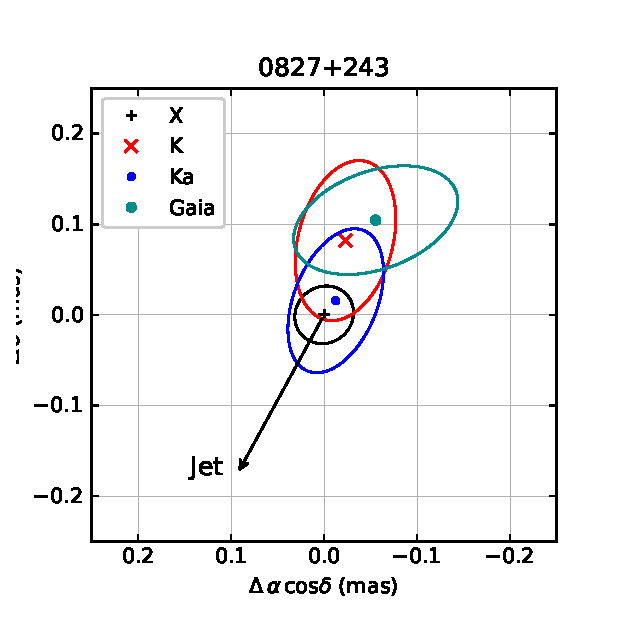
\includegraphics[width=\columnwidth]{figs/illustration-diagram2}
  \caption[]{\label{fig:illustration-diagram}
      Illustration diagram of calculation of position angle ($PA$) of offset vectors of $K$-band, $Ka$-band, and {\it Gaia} (optical) positions with respect to the $X$-band position for sources (top) 1157--215 and (bottom) 0827+243.
      The position angle is counted clockwise from the declination axis (Y-axis in the diagram).
      Also shown is the jet direction for these two sources taken from MOJAVE database \citep{2019ApJ...874...43L} for comparison whilst the magnitude (length) is arbitrary and thus meaningless.
  }
\end{figure}
%===========================================================================


%%%%%%%%%%%%%%%%%%%%%%%%%%%%%%%%%%%%%%%%%%%%%%%%%%%%%%%%%%%%%%%%%%%%%%%%%%%%
\section{Results}    \label{sec:result}
%%%%%%%%%%%%%%%%%%%%%%%%%%%%%%%%%%%%%%%%%%%%%%%%%%%%%%%%%%%%%%%%%%%%%%%%%%%%

%%%%%%%%%%%%%%%%%%%%%%%%%%%%%%%%%%%%%%%%%%%%%%%%%%%%%%%%%%%%%%%%%%%%%%%%%%%%
\subsection{Removal of large-scale differences}    \label{subsec:remove-sys}
%%%%%%%%%%%%%%%%%%%%%%%%%%%%%%%%%%%%%%%%%%%%%%%%%%%%%%%%%%%%%%%%%%%%%%%%%%%%

Table~\ref{tab:vsh01}-\ref{tab:vsh02} report the VSH parameters of the first and second degree, respectively.
The transformation parameters between $K$-band and $X$-band position are less than $30\,\mathrm{\mu as}$ except $D_2$ and $E_{21}^I$.
Similar results could be found in between $Ka$-band and $X$-band; however, significant terms, $D_3$, $E_{20}$, and $M_{20}$ exceeding 0.3~mas are also reported, which would cause a declination bias on the same level.
%This result justifies the necessity of removing the global difference and aligning the celestial frames at other wavelengths to the $X$-band frame before analyzing of position offsets.
Most of transformation parameters between \textit{Gaia} and $X$-band ranges from $30-50\,\mathrm{\mu as}$.

%
%% {tab:vsh01}
%===========================================================================
\begin{table*}[htbp]
    \centering
    \caption{\label{tab:vsh01}
        Rotation and glide and their formal uncertainties of ICRF3 $K$-band, $Ka$-band, and \textit{Gaia}-CRF2 catalogs with respect to the ICRF3 $X$-band catalog.
    }
    \begin{tabular}{cccccccc}
        \hline \noalign{\smallskip}
        &No. Sources & $R_1$ & $R_2$ & $R_3$ & $D_1$ & $D_2$ & $D_3$ \\
        & & $\mathrm{\mu as}$ & $\mathrm{\mu as}$  & $\mathrm{\mu as}$ & $\mathrm{\mu as}$ & $\mathrm{\mu as}$& $\mathrm{\mu as}$ \\
        \noalign{\smallskip}
        \hline 
        \noalign{\smallskip}
        $K - X$    & 793 &$ -15\pm  30$  &$-17 \pm  29$ &$+ 8 \pm  15$ &$-17 \pm  25$ &$+51 \pm  26$ &$+26 \pm  28$ \\
        $Ka - X$   & 638 &$ -27\pm  11$  &$- 2 \pm  11$ &$+17 \pm   7$ &$+ 7 \pm  10$ &$+35 \pm  10$ &$-354\pm  11$ \\
        $Gaia - X$ &2820 &$ +32 \pm 33$  &$-47 \pm  31$ &$-44 \pm  30$ &$-28 \pm  32$ &$+49 \pm  31$ &$-14 \pm  32$ \\
        \hline
    \end{tabular}
\end{table*}
%===========================================================================
%
%% {tab:vsh02}
%===========================================================================
\begin{table*}[htbp]
    \centering
    \caption{\label{tab:vsh02}
        Quadrupolar terms and their formal uncertainties of ICRF3 $K$-band, $Ka$-band, and \textit{Gaia}-CRF2 catalogs with respect to the ICRF3 $X$-band catalog.
    }
    \begin{tabular}{ccccccccccc}
        \hline \noalign{\smallskip}
        &$E_{22}^R$  &$E_{22}^I$  &$E_{21}^R$  &$E_{21}^I$  &$E_{20}$    &$M_{22}^R$  &$M_{22}^I$  &$M_{21}^R$  &$M_{21}^I$  &$M_{20}$    \\ 
        & $\mathrm{\mu as}$ & $\mathrm{\mu as}$  & $\mathrm{\mu as}$ & $\mathrm{\mu as}$ & $\mathrm{\mu as}$& $\mathrm{\mu as}$ & $\mathrm{\mu as}$ & $\mathrm{\mu as}$  & $\mathrm{\mu as}$ & $\mathrm{\mu as}$  \\
        \noalign{\smallskip}
        \hline
        \noalign{\smallskip}
        $K - X$      &$   -2 \pm    10 $  &$   -3 \pm    10 $  &$  -34 \pm    29 $  &$  -71 \pm    30 $  &$   +7 \pm    33 $  &$   +2 \pm    15 $  &$  -11 \pm    15 $  &$  +15 \pm    30 $  &$  -32 \pm    30 $  &$  -26 \pm    20 $ \\
        $Ka - X$  &$   -3 \pm     5 $  &$    5 \pm     5 $  &$  -33 \pm    12 $  &$   28 \pm    13 $  &$   86 \pm    13 $  &$   -1 \pm     6 $  &$  +10 \pm     6 $  &$   -7 \pm    11 $  &$   -2 \pm    12 $  &$  224 \pm    10 $ \\
        $Gaia - X$    &$  +37 \pm    19 $  &$   -3 \pm    19 $  &$  +9 \pm    37 $   &$  -50 \pm    40 $  &$  +41 \pm    36 $  &$   +2 \pm    20 $  &$   +1 \pm    20 $  &$  +26 \pm    38 $  &$  +72 \pm    39 $  &$  -12 \pm    33 $ \\
        \hline\end{tabular}
\end{table*}
%

Figure~\ref{fig:k-sx-pos-offset}-\ref{fig:gdr2-sx-pos-offset} present the position offset scatter of $K$-band, $Ka$-band, and \textit{Gaia} positions relative to the $X$-band position, as well as distributions of their right ascension and declination components for 488 common sources.
The agreement between $K$-band and $X$-band positions is around 0.1~mas on the right ascension;
The declination scatter is slightly larger, making the scatter cloud elongating along the declination axis.
This phenomenon is more pronounced between $Ka$-band and $X$-band.
The distribution of offset between \textit{Gaia} and $X$-band positions, with a nearly circle-like shape, is flatter than the $K$- and $Ka$-band, showing similar agreements of 0.3--0.5~mas on the right ascension and declination.
No bias larger than 0.1~mas in the right ascension and declination could be observed for all three position offsets.
As a result, we freed studies of multi-wavelength positions carried out in the next sections from large-scale differences. %due to deformations and alignment issues.

%% {fig:k-sx-pos-offset}
%===========================================================================
\begin{figure}[hbtp]
    \centering
    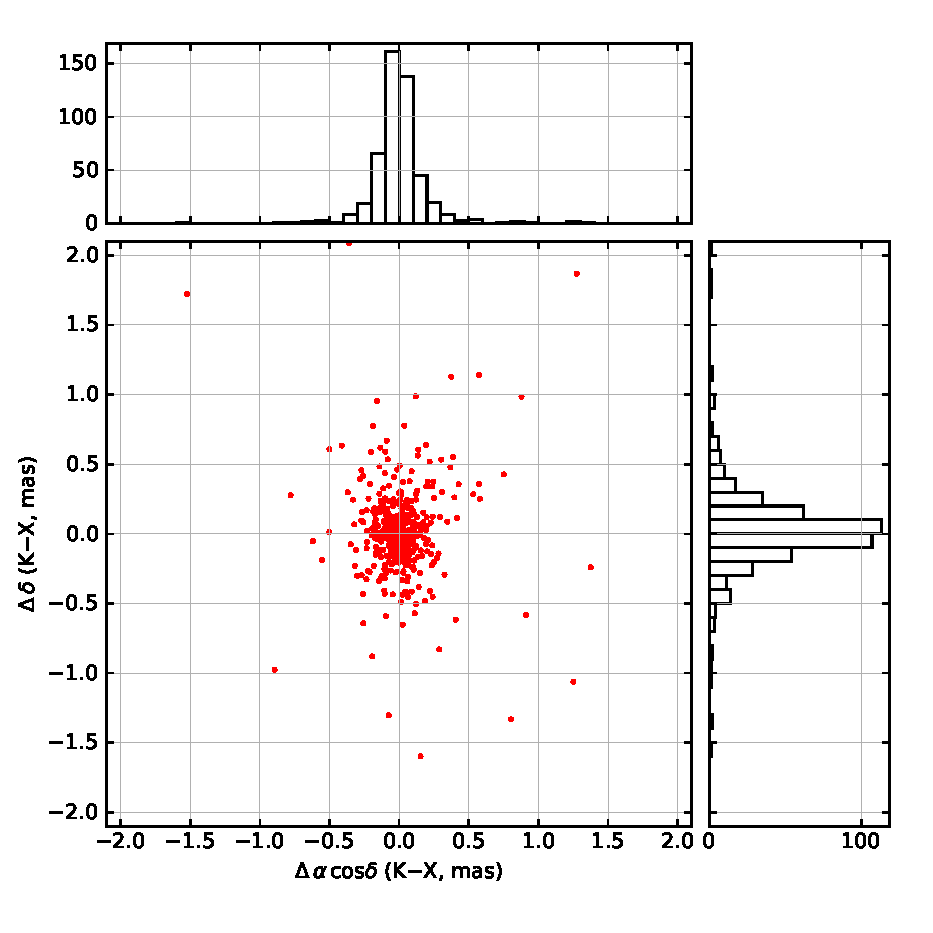
\includegraphics[width=\columnwidth]{figs/k-sx-scatter}
    \caption[]{\label{fig:k-sx-pos-offset}
        Position offset scatter and distribution of their component in the right ascension and declination for 488 sources between $X$- and $K$-band positions after removing the global differences, in the sense of ``K$-$X''.
    }
\end{figure}
%===========================================================================

%% {fig:xka-sx-pos-offset}
%===========================================================================
\begin{figure}[hbtp]
    \centering
    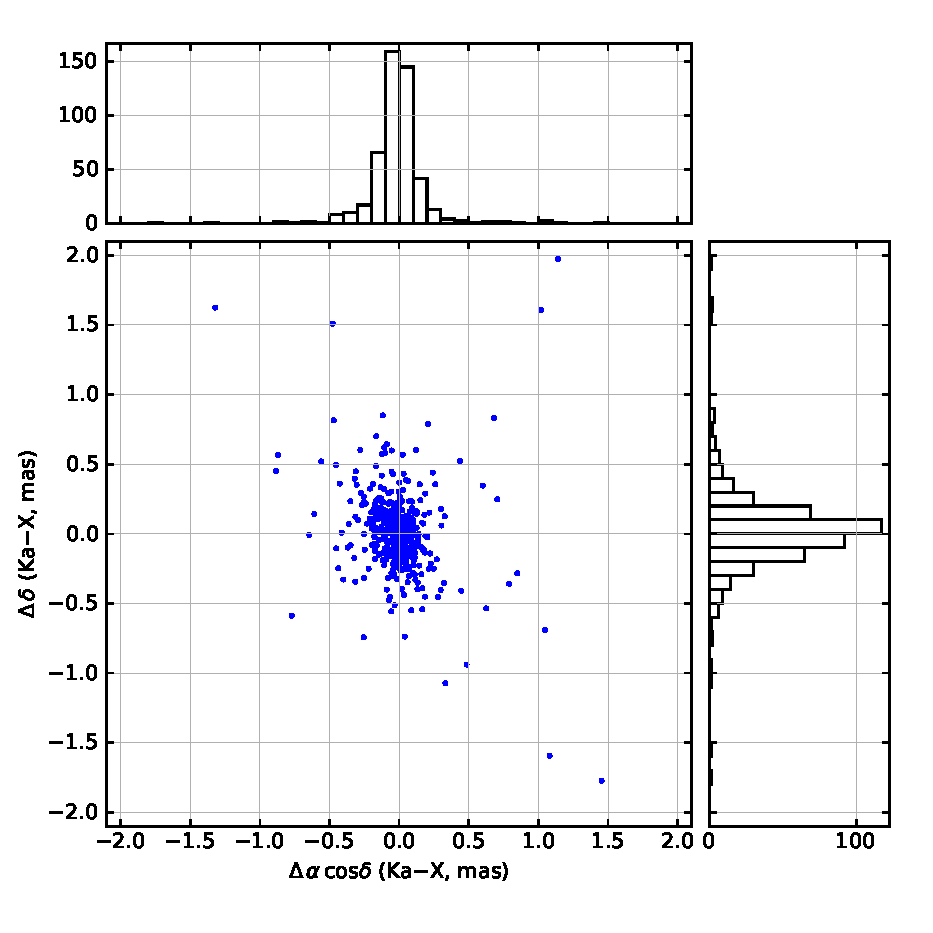
\includegraphics[width=\columnwidth]{figs/xka-sx-scatter}
    \caption[]{\label{fig:xka-sx-pos-offset}
        Position offset scatter and distribution of their component in the right ascension and declination for 488 sources between $X$- and $Ka$-band positions after removing the global differences, in the sense of ``Ka$-$X''.
    }
\end{figure}
%===========================================================================

%% {fig:gdr2-sx-pos-offset}
%===========================================================================
\begin{figure}[hbtp]
    \centering
    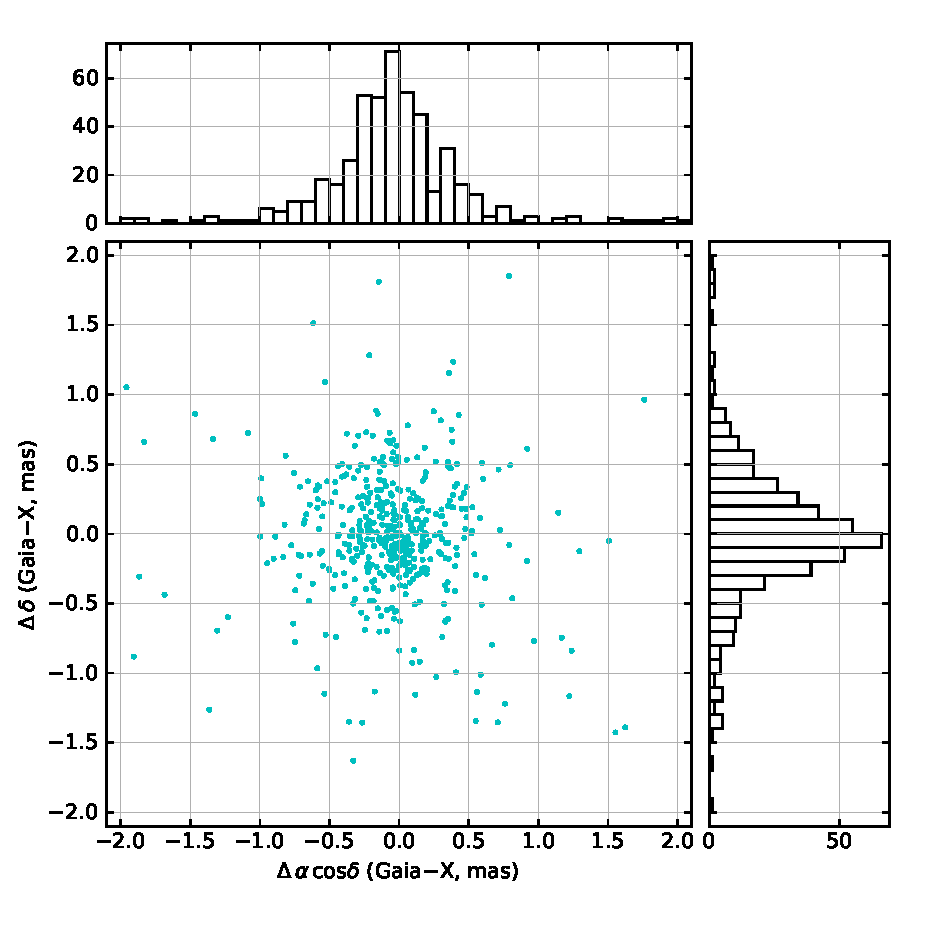
\includegraphics[width=\columnwidth]{figs/gaia-sx-scatter}
    \caption[]{\label{fig:gdr2-sx-pos-offset}
        Position offset scatter and distribution of their component in the right ascension and declination for 488 sources between $X$-band and {\it Gaia} positions after removing the global differences, in the sense of ``{\it Gaia}$-$X''.
    }
\end{figure}
%===========================================================================

%%%%%%%%%%%%%%%%%%%%%%%%%%%%%%%%%%%%%%%%%%%%%%%%%%%%%%%%%%%%%%%%%%%%%%%%%%%%
\subsection{Distribution of radio-to-optical offsets}    \label{subsec:r2o-dist}
%%%%%%%%%%%%%%%%%%%%%%%%%%%%%%%%%%%%%%%%%%%%%%%%%%%%%%%%%%%%%%%%%%%%%%%%%%%%

Figure~\ref{fig:rho-hist} depicts the distributions of radio-to-optical offsets, yielding a similar shape with an identical median value of 0.41~mas.
Only six sources have a radio-to-optical offset larger than 5~mas at either radio bands.
We found a second peak at around 0.6~mas at all three bands, which is sharpest at the $X$-band.

The distributions of normalized separations shown in Fig~\ref{fig:X-hist} are slightly different: it is sharper for the $Ka$-band while flatter for the $X$-band.
There are 16 sources at $X$-band, 6 at $K$-band, and 8 at $Ka$-band with $X~>~10$, which are beyond the axis.
Medians of normalized separations are 1.89, 1.69, and 1.77 for $X$-, $K$-, and $Ka$-band, respectively, all greater than the median value of 1.18 predicted from a Rayleigh distribution of unit standard deviation.
We fitted the normalized separation distributions to the Rayleigh curve with an unknown standard deviation $\sigma$.
The fitting returns the estimation of $\sigma$ to be 3.99 for $X$-band, 3.15 for $K$-band, and 3.21 for $Ka$-band. 
If we made a cut-off of 5 on the normalized separation, $\sigma$ is estimated to be 1.59 for $X$-band, 1.41 for $K$-band, and 1.46 for $Ka$-band. 
The distribution of $X$ would be closer to the Rayleigh shape if restricting sources to those with $X<3$, leaving out 138 sources to be outliers for $X$-band, 93 for $K$-band, and 92 for $K$-band.
% Outlier rate: 28% (X), 19% (K), 19% (Ka)

We further compared three radio-to-optical offsets of individual quasar, as presented in Fig~\ref{fig:rho-com}-\ref{fig:X-com}.
Except for few cases, the radio-to-optical offsets determined from $X$-, $K$-, and $Ka$-band generally agrees with each other.
%No statistically obvious evidence shows that the radio-to-optical offset decreases at high frequency.
Further examinations report 443 sources (~91\%) with an absolute difference less than 0.5~mas among three radio-to-optical offsets.
We observed similar results for normalized separations, regardless the normalized separation at $X$-band is slightly statistically larger than other two bands.

For individual sources, radio-to-optical offsets might be significantly inconsistently.
We listed four groups of interest as listed below and discussed them in Sect.~\ref{subsec:cause-of-VG}.
%
\begin{enumerate}
    \item[A] 45 sources with radio-to-radio offsets < 0.5~mas, radio-to-optical offsets > 1~mas.
    \item[B] 2 sources with $X$-\textit{Gaia} offset > 1~mas, $K$-\textit{Gaia} and $Ka$-\textit{Gaia} offset < 0.5~mas.
    They are 0723--008 and 2134+004.
    \item[C] 2 sources with $Ka$-\textit{Gaia} offset > 1~mas, $X$-\textit{Gaia} and $K$-\textit{Gaia} offset < 0.5~mas.
    They are 1315--058 and 1437+374.
    \item[D] 2 sources with $K$-\textit{Gaia} offset > 1~mas, $X$-\textit{Gaia} and $Ka$-\textit{Gaia} offset < 0.5~mas.
    They are 0430--332 and 1611-710.
\end{enumerate}
%
%For example, 2008--159 has an angular separation of $\sim\mathrm{0.2~mas}$ between $X$-band and \textit{Gaia}, $\sim\mathrm{0.1~mas}$ between $Ka$-band and \textit{Gaia} but a few micro-arcseconds for between $K$-band and \textit{Gaia}.
%It suggests that VLBI at $X$-band and $Ka$-band measures the same or close emission center while $K$-band VLBI and \textit{Gaia} measures another one.
%Similar cases could be found, such as 0827+243 with $\rho~(\rm $K$-Gaia) \simeq~\rho~(\rm $Ka$-Gaia)~\simeq~0.01~{\rm mas}$ but $\rho~(\rm $X$-Gaia) \simeq~0.1~{\rm mas}$, 
%and 1315--058 with $\rho\,(\rm $K$-Gaia)\,\simeq~\rho~(\rm $X$-Gaia)~\simeq~0.3~{\rm mas}$ but $\rho~(\rm $Ka$-Gaia) \simeq~13.6~{\rm mas}$.

%% {fig:rho-hist}
%===========================================================================
\begin{figure}[hbtp]
    \centering
    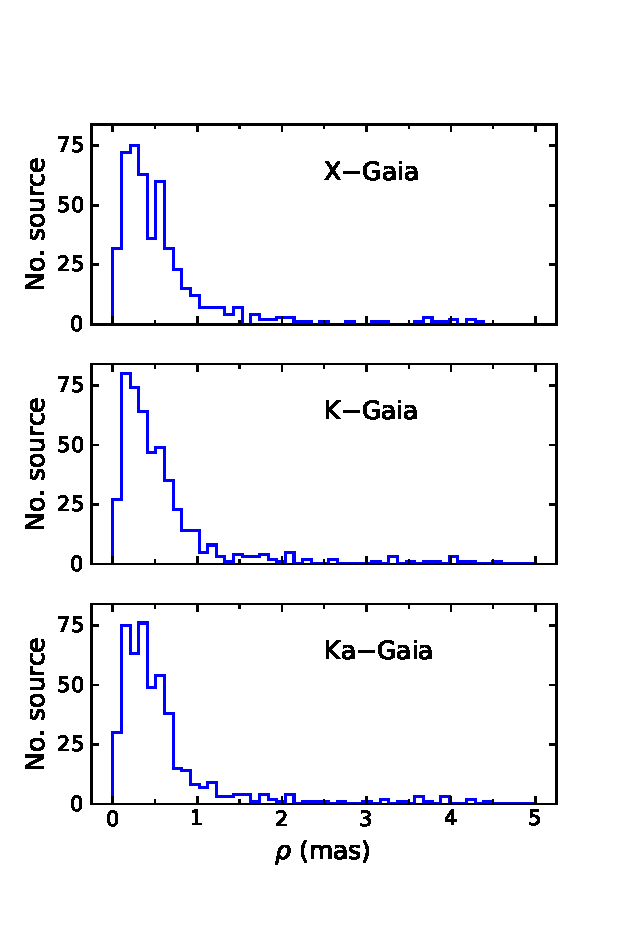
\includegraphics[width=\columnwidth]{figs/rho-hist}
    \caption[]{\label{fig:rho-hist}
        Distribution of angular separation $\rho$ between the {\it Gaia} position and VLBI positions at $X$-, $K$-, and $Ka$-band for 488 sources.
    }
\end{figure}
%===========================================================================

%% {fig:X-hist}
%===========================================================================
\begin{figure}[hbtp]
    \centering
    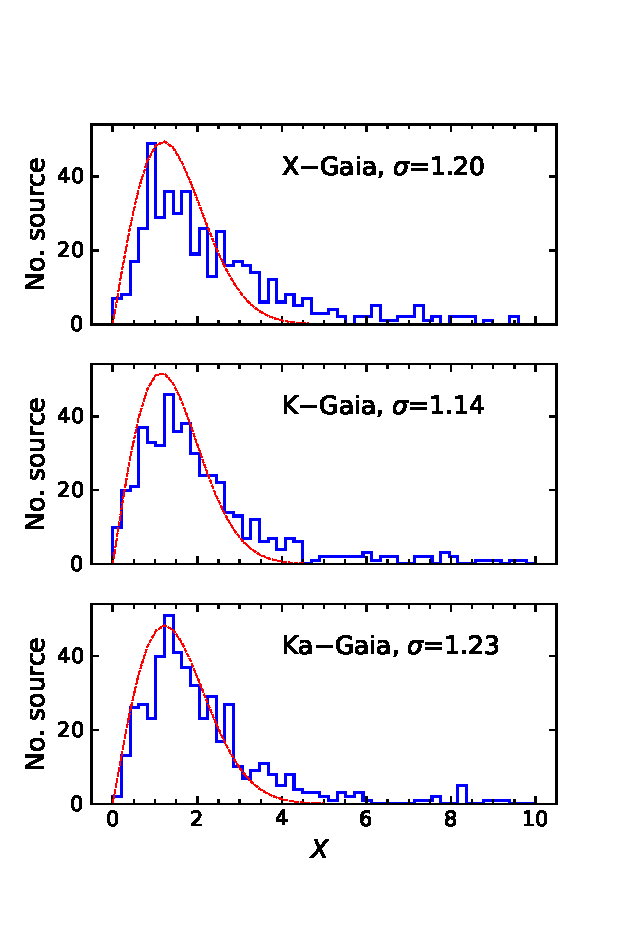
\includegraphics[width=\columnwidth]{figs/X-hist}
    \caption[]{\label{fig:X-hist}
        Distribution of normalized separation $X$ between the {\it Gaia} position and VLBI positions at $X$-, $K$-, and $Ka$-band for 488 sources.
        The red dashed curves represent standard Rayleigh distributions with a standard deviation of 1.59, 1.41, and 1.46, from top to bottom, respectively.
    }
\end{figure}
%===========================================================================


%% {fig:rho-com}
%===========================================================================
\begin{figure}[hbtp]
    \centering
    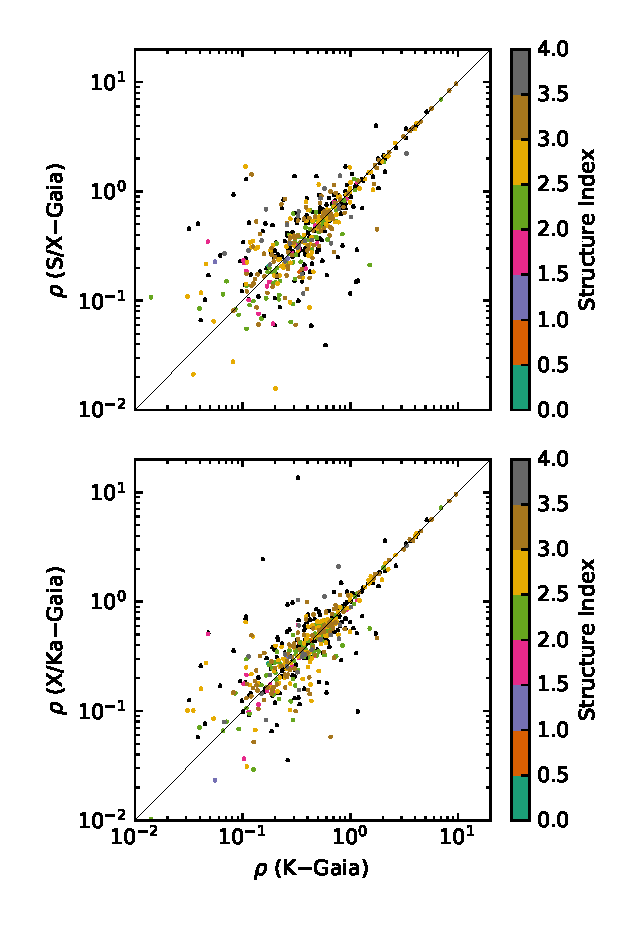
\includegraphics[width=\columnwidth]{figs/rho-com-vs-si}
    \caption[]{\label{fig:rho-com}
        Distribution of angular separation $\rho$ between the {\it Gaia} position and VLBI positions at $X$-, $K$-, and $Ka$-band for 488 sources.
        The red circles represents 322 sources having a structure index at $X$-band in the BVID database with the color codes tracing the value of the structure index, while black triangles stand for the other 166 sources.
    }
\end{figure}
%===========================================================================

%% {fig:X-com}
%===========================================================================
\begin{figure}[hbtp]
    \centering
    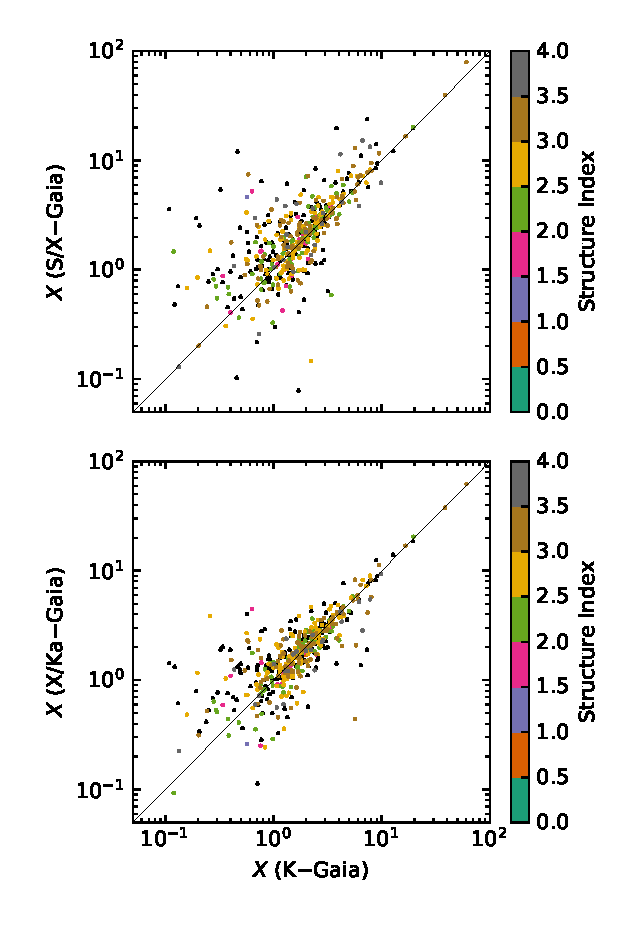
\includegraphics[width=\columnwidth]{figs/X-com-vs-si}
    \caption[]{\label{fig:X-com}
        Distribution of normalized separation $X$ between the {\it Gaia} position and VLBI positions at $X$-, $K$-, and $Ka$-band for 488 sources.
        The red circles represents 322 sources having a structure index at $X$-band in the BVID database with the color codes tracing the value of the structure index, while black triangles stand for the other 166 sources.
    }
\end{figure}
%===========================================================================

%%%%%%%%%%%%%%%%%%%%%%%%%%%%%%%%%%%%%%%%%%%%%%%%%%%%%%%%%%%%%%%%%%%%%%%%%%%%
\subsection{Correlation between radio-to-optical offsets and astrophysical parameters}    \label{subsec:r2o-corr}
%%%%%%%%%%%%%%%%%%%%%%%%%%%%%%%%%%%%%%%%%%%%%%%%%%%%%%%%%%%%%%%%%%%%%%%%%%%%

Then we studied the correlation between radio-to-optical offsets with astrophysical properties.
The radio structure index of 322 sources is color-coded in the Figs.~\ref{fig:rho-com}-\ref{fig:X-com}, where we could not detect a obvious correlation. % between the radio-to-optical offsets.
For most sources, the structure index falls in the range of 2 to 3.5.

Figure~\ref{fig:rho-g-mag} demonstrates a correlation between the radio-to-optical offsets and \textit{Gaia} $G$ magnitude: the radio-to-optical offsets increase towards the faint end for all three radio bands.
This correlation could be still seen if we included all the common sources between each ICRF catalog and \textit{Gaia}-CRF2 subsets, for instance, the 2820 sources between the ICRF3 $X$-band catalog and \textit{Gaia}-CRF2.
We also plotted the normalized separation against the $G$ magnitude in the Fig.~\ref{fig:$X$-g-mag} and found a slightly decreasing trend for $X$-band and flat trends for $K$- and $Ka$-band at $17\,<\,G\,<\,20$.
We did not detect any dependency of neither radio-to-optical angular separation (Fig.~\ref{fig:rho-z}) nor normalized separation (not plotted for brevity) on the redshift.


All three morphological indices larger than one were found for 
9 sources at the filter $B$, 16 sources at the filter $R$, and 25 sources at the filter $IR$, corresponding to about 5\%, 4\% and 7\% of the subset with these morphological indices available, respectively.
Figures~\ref{fig:rho-I1R}-\ref{fig:rho-I3R} demonstrates a smooth dependency of the radio-to-optical distance on the three morphological index of $R$-filter.
The morphological index of filter $B$ and $IR$ present similar results to those of filter $R$ and thus are not plotted here.


%% {fig:rho-g-mag}
%===========================================================================
\begin{figure}[hbtp]
    \centering
    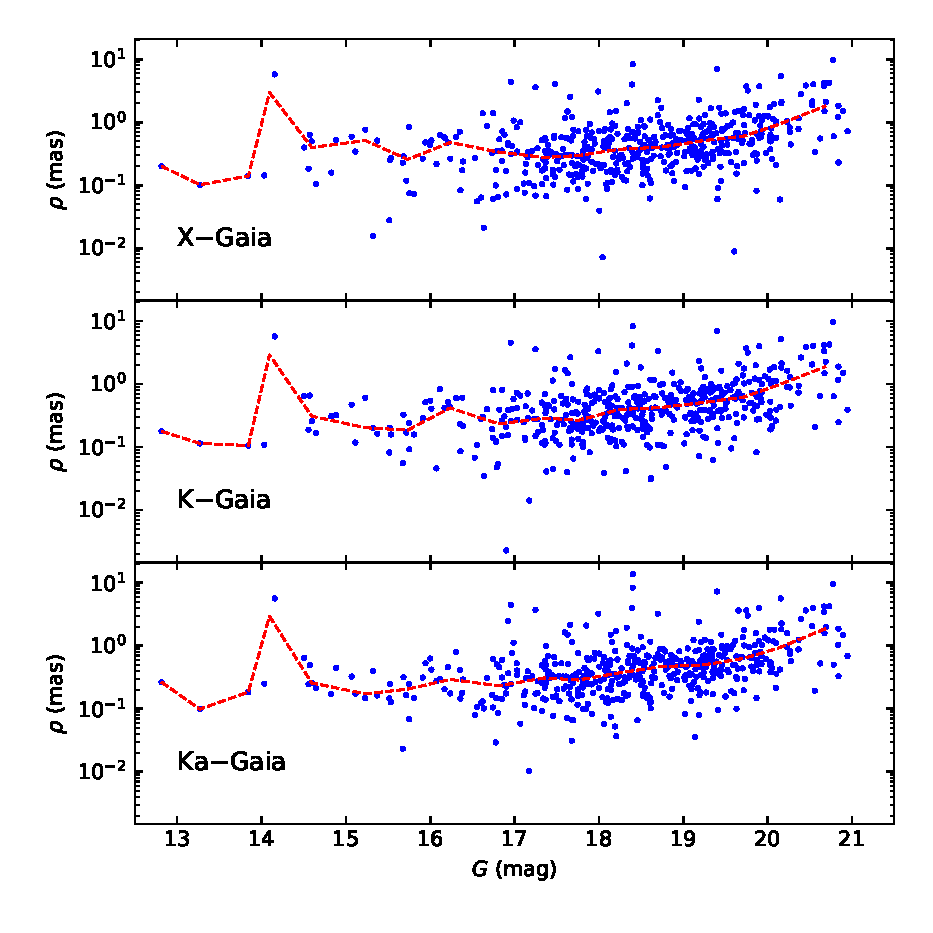
\includegraphics[width=\columnwidth]{figs/rho-g-mag}
    \caption[]{\label{fig:rho-g-mag}
        Angular separation $\rho$ between the {\it Gaia} position and VLBI positions at $X$-, $K$-, and $Ka$-band as a function of \textit{Gaia} $G$ magnitude for 488 sources.
        The red dashed line indicates the median values in subsets binned by a step of 0.5~mag.
    }
\end{figure}
%===========================================================================

%% {fig:X-g-mag}
%===========================================================================
\begin{figure}[hbtp]
    \centering
    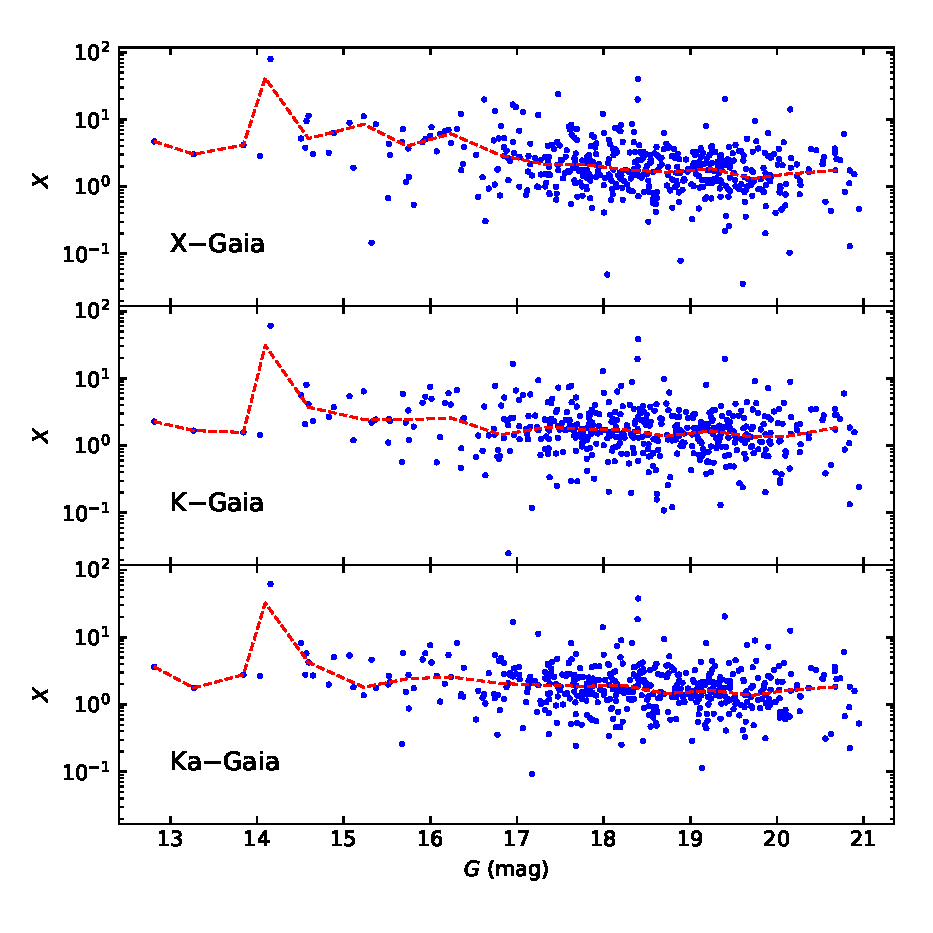
\includegraphics[width=\columnwidth]{figs/X-g-mag}
    \caption[]{\label{fig:$X$-g-mag}
        Normalized separation $X$ between the {\it Gaia} position and VLBI positions at $X$-, $K$-, and $Ka$-band as a function of \textit{Gaia} $G$ magnitude for 488 sources.
        The red dashed line indicates the median values in subsets binned by a step of 0.5~mag.
    }
\end{figure}
%===========================================================================

%% {fig:rho-z}
%===========================================================================
\begin{figure}[hbtp]
    \centering
    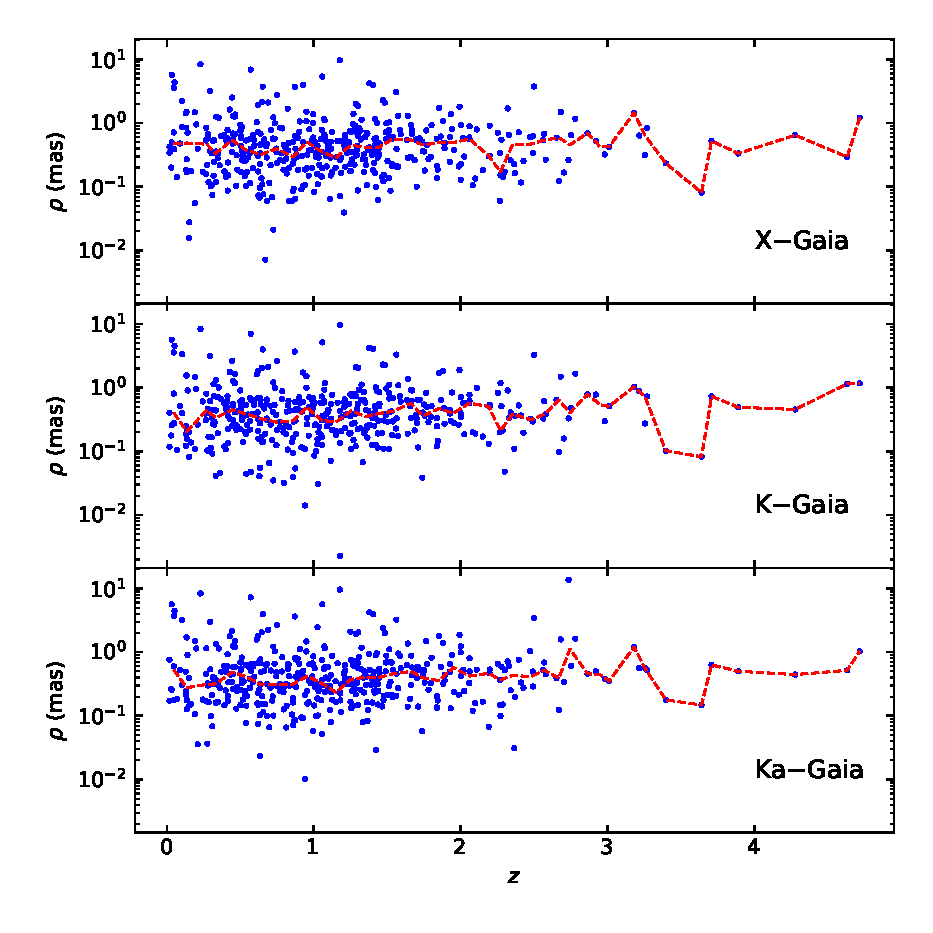
\includegraphics[width=\columnwidth]{figs/rho-z}
    \caption[]{\label{fig:rho-z}
        Angular separation $\rho$ between the {\it Gaia} position and VLBI positions at $X$-, $K$-, and $Ka$-band as a function of red-shift $z$ for 443 sources having a red-shift measurements in the LQAC-5 catalog.
        The red dashed line indicates the median values in subsets binned by a step of 0.1.
    }
\end{figure}
%===========================================================================

%% {fig:rho-I1R}
%===========================================================================
\begin{figure}[hbtp]
    \centering
    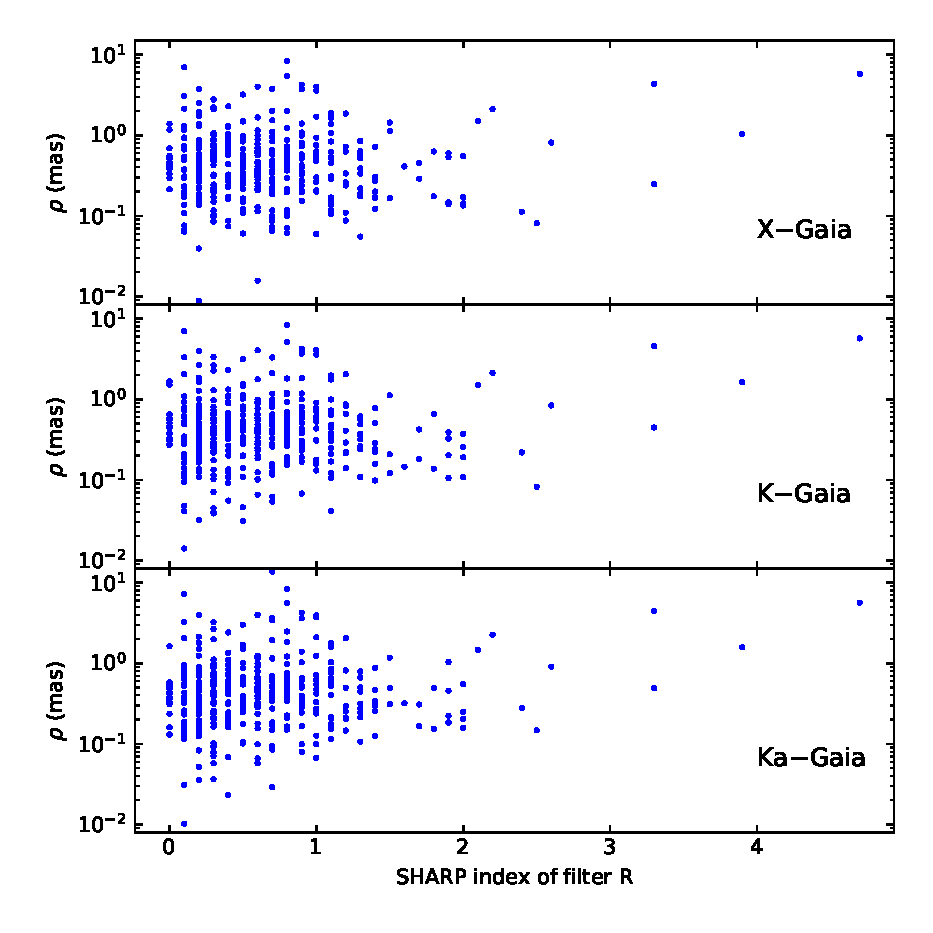
\includegraphics[width=\columnwidth]{figs/rho-I1R}
    \caption[]{\label{fig:rho-I1R}
        Angular separation $\rho$ between the {\it Gaia} position and VLBI positions at $X$-, $K$-, and $Ka$-band as a function of morphological SHARP index at filter R for 396 sources having R-filter morphological indices in the LQAC-5 catalog.
    }
\end{figure}
%===========================================================================

%% {fig:rho-I2R}
%===========================================================================
\begin{figure}[hbtp]
    \centering
    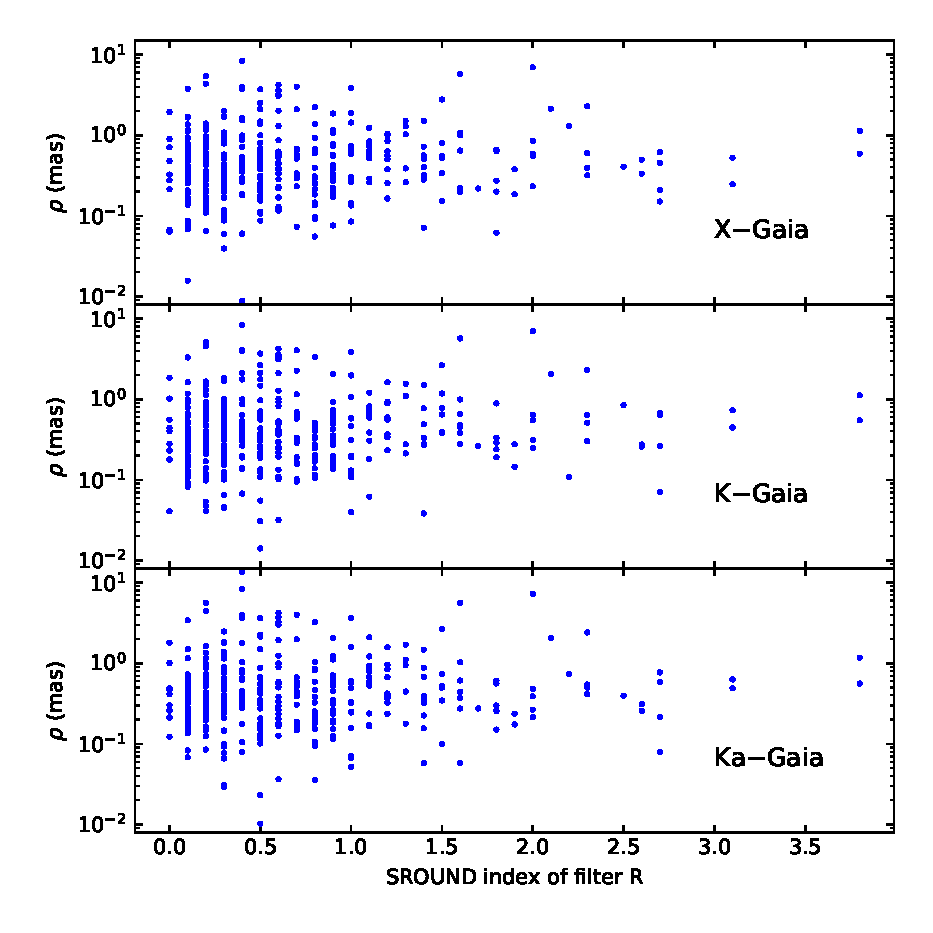
\includegraphics[width=\columnwidth]{figs/rho-I2R}
    \caption[]{\label{fig:rho-I2R}
        Angular separation $\rho$ between the {\it Gaia} position and VLBI positions at $X$-, $K$-, and $Ka$-band as a function of morphological SROUND index at filter R for 396 sources having R-filter morphological indices in the LQAC-5 catalog.
    }
\end{figure}
%===========================================================================

%% {fig:rho-I3R}
%===========================================================================
\begin{figure}[hbtp]
    \centering
    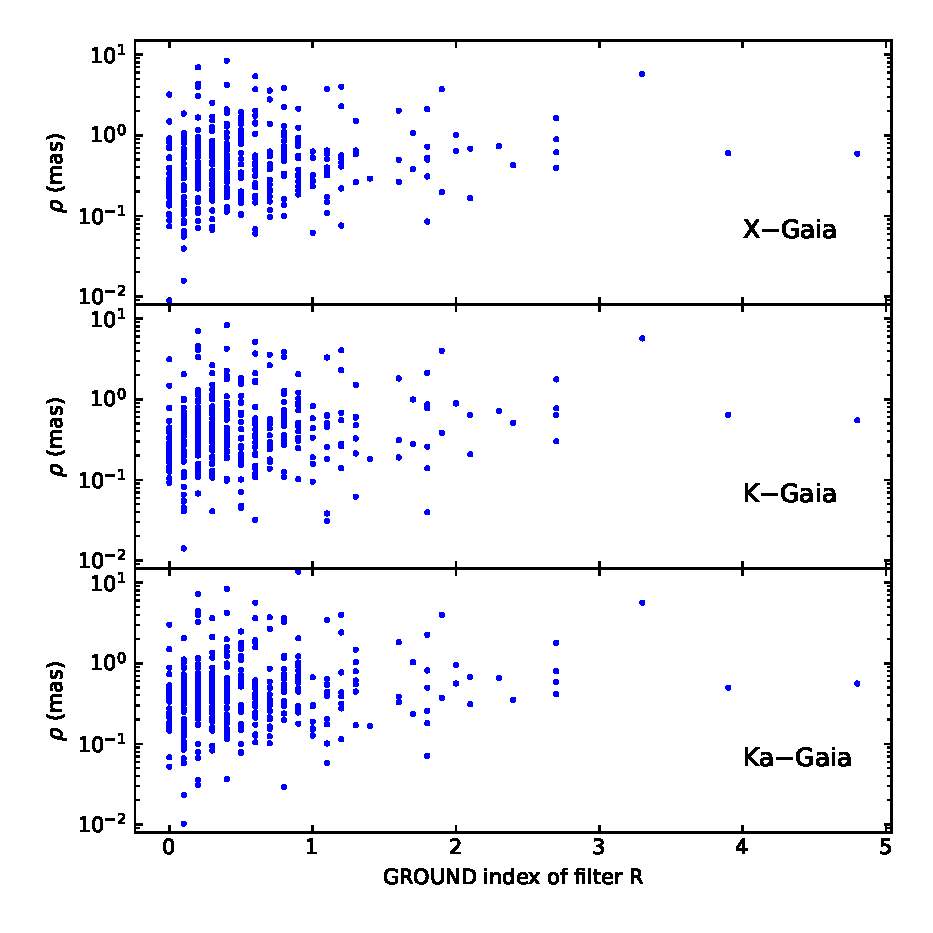
\includegraphics[width=\columnwidth]{figs/rho-I3R}
    \caption[]{\label{fig:rho-I3R}
        Angular separation $\rho$ between the {\it Gaia} position and VLBI positions at $X$-, $K$-, and $Ka$-band as a function of morphological GROUND index at filter R for 340 sources having R-filter morphological indices in the LQAC-5 catalog.
    }
\end{figure}
%===========================================================================

%%%%%%%%%%%%%%%%%%%%%%%%%%%%%%%%%%%%%%%%%%%%%%%%%%%%%%%%%%%%%%%%%%%%%%%%%%%%
\subsection{Aligned multi-wavelength positions}    \label{subsec:pos-align}
%%%%%%%%%%%%%%%%%%%%%%%%%%%%%%%%%%%%%%%%%%%%%%%%%%%%%%%%%%%%%%%%%%%%%%%%%%%%

In this section, we used the direction information of the position offset to investigate the relation of multi-wavelength positions for individual source.
The position angles of $K$-band, $Ka$-band, and \textit{Gaia} positions with referred to the $X$-band position are plotted in Fig.~\ref{fig:pa-hist}.
Peaks at around $0\,^\circ$, $180\,^\circ$, and $360\,^\circ$ could be observed for $K$- and $Ka$-band positions, while \textit{Gaia} position does not show a similar preference.

In order to compare the position angles of $K$-band, $Ka$-band, and \textit{Gaia} positions with respective to the $X$-band position,
we calculated the absolute differences between these position angles and wrapped them into the range of $0-180^\circ$.
Figure~\ref{fig:pa-diff} depicts the distribution of position angle differences, where one could observe a clear peak around $0^\circ$ above the mean value (red dashed line) while no peak appears at $180^\circ$.
If we set a limit on the position angle difference, below which the multi-wavelength positions could be considered as aligned, the number of sources for different cases is summarized in the Table~\ref{tab:no_sou_aligned}.
Note that only for sources with all (at least two) normalized separations $X>1$ with respective to the $X$-band position, the derived position angle is reliable.
Taking this conditions into consideration reduces the subset of sources with aligned positions to nearly their half-size.

We adopted a limit of $30^\circ$ on the PA difference and the condition of $X>1$ for further analysis.
As a result, we obtained a sample of 54 sources having positions at  four frequencies aligned, among which we found the jet information for 23 sources from \citep{2019ApJ...874...43L}.
Figure~\ref{fig:jet-pa-com} depicts the distribution of the absolute difference between the jet direction and \textit{Gaia}--X offset vector.
Again, we considered a PA difference limit of $30^\circ$, therefore, 7 sources have the radio-to-optical offset in the downstream direction while 6 sources with PA difference yields a radio-to-optical offset in the upstream of the jet.
Table~\ref{tab:aligned-sou} tabulates the position offsets of $K$-band, $Ka$-band, and \textit{Gaia} positions with respective to the $X$-band position for 54 sources whose four-band positions are aligned. %, as well as the jet direction if available. 

%% {fig:pa-hist}
%===========================================================================
\begin{figure}[hbtp]
    \centering
    \includegraphics[width=\columnwidth]{figs/pa-hist}
    \caption[]{\label{fig:pa-hist}
        Distribution of the position angle of offset vector of $K$-band, $Ka$-band, and \textit{Gaia} positions with referred to the $X$-band position for 488 common sources.
        The horizontal red dashed line stands for a uniform distribution.
    }
\end{figure}
%===========================================================================

%% {fig:pa-diff}
%===========================================================================
\begin{figure}[hbtp]
    \centering
    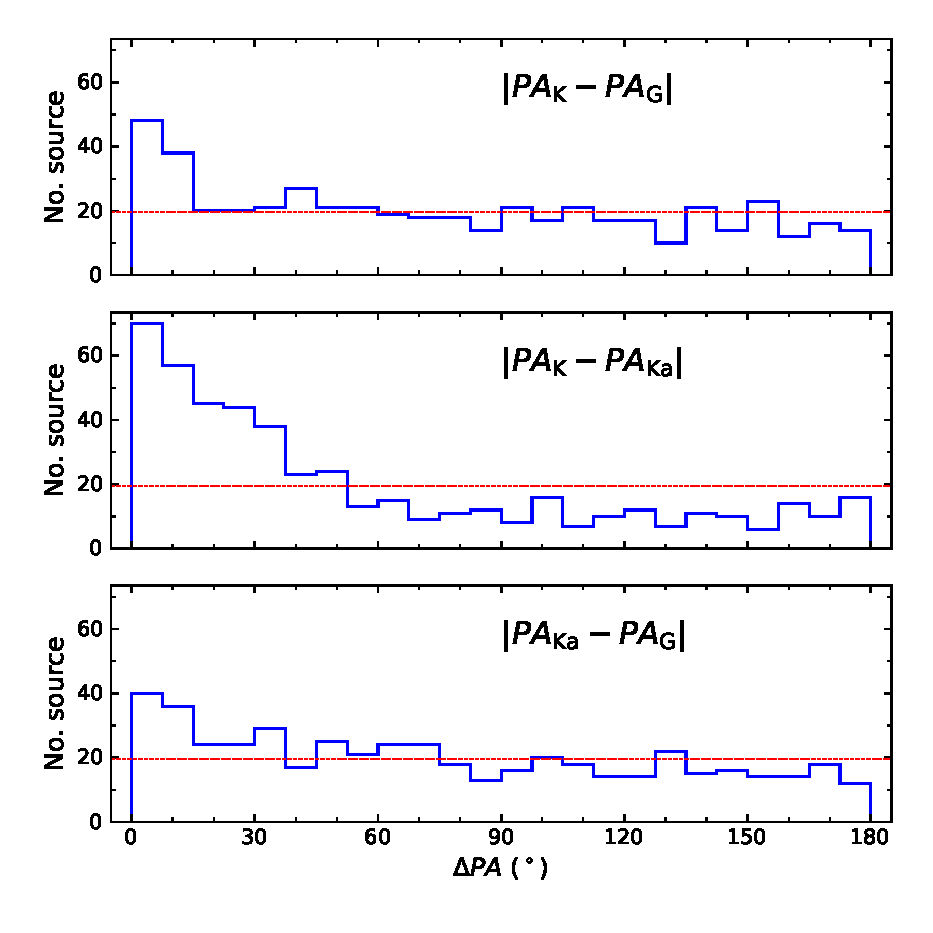
\includegraphics[width=\columnwidth]{figs/pa-diff}
    \caption[]{\label{fig:pa-diff}
        Distribution of the absolute position angle difference of offset vector of $K$-band, $Ka$-band, and \textit{Gaia} positions with referred to the $X$-band position for 488 common sources. 
        The horizontal red dashed line stands for a uniform distribution.
    }
\end{figure}
%===========================================================================

%% {fig:jet-pa-co}
%===========================================================================
\begin{figure}[hbtp]
    \centering
    \includegraphics[width=\columnwidth]{figs/jet-pa-com}
    \caption[]{\label{fig:jet-pa-com}
        Distribution of the absolute position angle difference of $K$--X position offset vector and jet vector for 23 sources whose four-band positions are almost aligned ($\Delta~PA~<~30^{\circ}$).
    }
\end{figure}
%===========================================================================

%
%% {tab:no_sou_aligned}
%===========================================================================
\begin{table*}[htbp]
    \centering
    \caption{\label{tab:no_sou_aligned}
        Number of sources with multi-wavelength positions aligned.
    }
    \begin{tabular}{ccccc}
        \hline \noalign{\smallskip}
        &$X$, $K$, $Ka$ &$X$, $K$, \textit{\it Gaia} &$X$, $Ka$, \textit{\it Gaia} &$X$, $K$, $Ka$, \textit{\it Gaia}\\
        \noalign{\smallskip}
        \hline 
        \noalign{\smallskip}
        $\Delta PA<45^\circ$       &277  &174  &170  &99\\
        $\Delta PA<30^\circ$       &216  &126  &124  &63\\     
        $\Delta PA<15^\circ$       &127  &87   &76   &30\\
        $\Delta PA<45^\circ, X<1$  &171  &96   &110  &78\\
        $\Delta PA<30^\circ, X<1$  &135  &74   &85   &54\\
        $\Delta PA<15^\circ, X<1$  &87   &52   &56   &28\\
        \hline
    \end{tabular}
\end{table*}
%===========================================================================

%% {tab:aligned-sou}
%===========================================================================
\begin{table*}
    \centering
        \caption{\label{tab:aligned-sou}
        Sources with positions at four bands aligned within $30~^\circ$.
    }
    \begin{tabular}{ccccccccccccccc}
    \hline \noalign{\smallskip}
        IERS name & $\rho_{\rm K}$ & $PA_{\rm K}$ & $X_{\rm K}$ & $\rho_{\rm Ka}$ & $PA_{\rm Ka}$ & $X_{\rm Ka}$ & $\rho_{\rm G}$ & $PA_{\rm G}$ & $X_{\rm G}$ & $PA_{\rm jet}$ & SI & SHARP & SROUND & GROUND \\
        & $\mathrm{mas}$ & $\mathrm{{}^{\circ}}$ &  & $\mathrm{mas}$ & $\mathrm{{}^{\circ}}$ &  & $\mathrm{mas}$ & $\mathrm{{}^{\circ}}$ & $\mathrm{mas}$ & $\mathrm{{}^{\circ}}$ &  &  &  &  \\
        \hline \noalign{\smallskip}
        % Downstream
        0859-140 & 0.3 & 3.1 & 198 & 0.2 & 2.4 & 207 & 0.3 & 3.0 & 195 & 178 & 4.1 & 0.9 & 0.4 & 0.2 \\
        1034-293 & 0.1 & 0.6 & 151 & 0.1 & 1.3 & 132 & 0.5 & 3.7 & 140 & 148 & 2.4 & 1.1 & 0.3 & 0.3 \\
        1157-215 & 2.3 & 10.0 & 318 & 3.6 & 8.4 & 319 & 4.0 & 23.9 & 316 & 324 & - & - & - & - \\
        1222+216 & 0.2 & 2.1 & 11 & 0.1 & 1.0 & 29 & 0.5 & 6.3 & 359 & 13 & - & 1.3 & 0.7 & 0.9 \\
        1742-078 & 0.4 & 1.6 & 186 & 0.3 & 1.2 & 187 & 1.1 & 2.6 & 189 & 169 & 3.2 & - & - & - \\
        2029+121 & 0.1 & 1.6 & 199 & 0.2 & 1.8 & 173 & 0.7 & 1.4 & 201 & 183 & - & - & - & - \\
        2134+004 & 1.1 & 17.2 & 123 & 1.3 & 15.4 & 123 & 1.4 & 19.8 & 123 & 96 & - & 0.0 & 0.5 & 0.4 \\
        \hline \noalign{\smallskip}
        % Upstream
        0430+052 & 0.7 & 12.9 & 58 & 0.7 & 12.0 & 60 & 0.5 & 11.4 & 76 & 258 & 4.2 & 0.3 & 2.6 & 1.8 \\
        0723-008 & 1.6 & 15.5 & 149 & 1.9 & 19.3 & 146 & 1.4 & 7.5 & 148 & 343 & 3.3 & 1.5 & 1.0 & 0.6 \\
        0743-006 & 0.3 & 3.4 & 220 & 1.0 & 14.3 & 233 & 1.0 & 12.9 & 230 & 42 & 3.2 & 0.6 & 1.6 & 0.1 \\
        0827+243 & 0.1 & 1.3 & 336 & 0.1 & 1.3 & 334 & 0.1 & 1.5 & 338 & 152 & 2.5 & 0.1 & 0.5 & 0.1 \\
        0850+581 & 0.8 & 6.4 & 321 & 0.5 & 3.7 & 325 & 0.8 & 7.2 & 337 & 153 & 3.2 & 0.3 & 0.2 & 0.2 \\
        1038+064 & 0.2 & 2.0 & 348 & 0.2 & 2.1 & 350 & 0.4 & 3.8 & 344 & 137 & 3.7 & - & - & - \\
        \hline \noalign{\smallskip}
        % Other
        0112-017 & 0.6 & 7.6 & 265 & 0.6 & 6.9 & 283 & 0.7 & 4.4 & 278 & 146 & 4.2 & 0.2 & 0.1 & 0.3 \\
        0122-003 & 0.5 & 2.5 & 329 & 0.9 & 4.2 & 352 & 0.6 & 3.4 & 358 & 276 & - & 1.0 & 1.1 & 0.8 \\
        0430+052 & 0.7 & 12.9 & 58 & 0.7 & 12.0 & 60 & 0.5 & 11.4 & 76 & 258 & 4.2 & 0.3 & 2.6 & 1.8 \\
        0528+134 & 0.1 & 2.5 & 279 & 0.1 & 1.6 & 280 & 0.9 & 1.3 & 269 & 32 & 2.5 & 0.6 & 0.3 & 2.7 \\
        0552+398 & 0.1 & 1.7 & 324 & 0.2 & 2.8 & 323 & 0.2 & 1.9 & 327 & 358 & 2.7 & 0.1 & 0.3 & 0.2 \\
        0723-008 & 1.6 & 15.5 & 149 & 1.9 & 19.3 & 146 & 1.4 & 7.5 & 148 & 343 & 3.3 & 1.5 & 1.0 & 0.6 \\
        0743-006 & 0.3 & 3.4 & 220 & 1.0 & 14.3 & 233 & 1.0 & 12.9 & 230 & 42 & 3.2 & 0.6 & 1.6 & 0.1 \\
        0827+243 & 0.1 & 1.3 & 336 & 0.1 & 1.3 & 334 & 0.1 & 1.5 & 338 & 152 & 2.5 & 0.1 & 0.5 & 0.1 \\
        0850+581 & 0.8 & 6.4 & 321 & 0.5 & 3.7 & 325 & 0.8 & 7.2 & 337 & 153 & 3.2 & 0.3 & 0.2 & 0.2 \\
        0859-140 & 0.3 & 3.1 & 198 & 0.2 & 2.4 & 207 & 0.3 & 3.0 & 195 & 178 & 4.1 & 0.9 & 0.4 & 0.2 \\
        0917+449 & 0.3 & 3.2 & 173 & 0.3 & 3.6 & 160 & 0.3 & 3.1 & 148 & 197 & 2.7 & 1.0 & 1.0 & 0.2 \\
        0953+254 & 0.3 & 4.2 & 23 & 0.3 & 4.5 & 32 & 0.8 & 4.3 & 49 & 264 & 3.2 & 0.4 & 0.1 & 0.5 \\
        1034-293 & 0.1 & 0.6 & 151 & 0.1 & 1.3 & 132 & 0.5 & 3.7 & 140 & 148 & 2.4 & 1.1 & 0.3 & 0.3 \\
        1038+064 & 0.2 & 2.0 & 348 & 0.2 & 2.1 & 350 & 0.4 & 3.8 & 344 & 137 & 3.7 & - & - & - \\
        1157-215 & 2.3 & 10.0 & 318 & 3.6 & 8.4 & 319 & 4.0 & 23.9 & 316 & 324 & - & - & - & - \\
        1222+216 & 0.2 & 2.1 & 11 & 0.1 & 1.0 & 29 & 0.5 & 6.3 & 359 & 13 & - & 1.3 & 0.7 & 0.9 \\
        1611+343 & 0.3 & 5.1 & 202 & 0.2 & 2.4 & 198 & 0.3 & 4.1 & 180 & 113 & 3.1 & 0.4 & 0.5 & 0.1 \\
        1742-078 & 0.4 & 1.6 & 186 & 0.3 & 1.2 & 187 & 1.1 & 2.6 & 189 & 169 & 3.2 & - & - & - \\
        2029+121 & 0.1 & 1.6 & 199 & 0.2 & 1.8 & 173 & 0.7 & 1.4 & 201 & 183 & - & - & - & - \\
        2113+293 & 0.1 & 1.7 & 253 & 0.1 & 1.2 & 230 & 0.8 & 3.1 & 247 & 198 & - & 0.4 & 0.9 & 0.3 \\
        2134+004 & 1.1 & 17.2 & 123 & 1.3 & 15.4 & 123 & 1.4 & 19.8 & 123 & 96 & - & 0.0 & 0.5 & 0.4 \\
        2234+282 & 0.4 & 6.3 & 225 & 0.3 & 5.4 & 221 & 0.5 & 3.0 & 224 & 151 & - & 0.2 & 0.6 & 0.6 \\
        2251+158 & 0.4 & 7.2 & 76 & 0.3 & 4.4 & 69 & 0.5 & 8.5 & 70 & 280 & - & 0.1 & 0.7 & 0.5 \\
        \hline \noalign{\smallskip}
    \end{tabular}
    \tablefoot{
    Sources are divided into three groups:
    (Top) \textit{Gaia} positions in the downstream of jet with respect to the $X$-band positions;
    (Middle) \textit{Gaia} positions in the upstream of jet;
    (Bottom) others.
    The first column gives the source name of IERS designation .
    The columns 2-4, 5-7, 8-10 present the angular separation $\rho$, normalized separation $X$, and position angle of $K$-X, $Ka$-X, and \textit{Gaia}-X offset.
    The column 11 contains the jet direction collected from the Table~4 in \citet{2019ApJ...874...43L}, followed by the source structure index provided by BVID database.
    The last three columns list the morphological index, namely, SHARP, SROUND, and GROUND, at R filter taken from the LQAC-5 catalog.
    The ``-'' symbol means that the corresponding information is not available.
}
\end{table*}

%===========================================================================

%%%%%%%%%%%%%%%%%%%%%%%%%%%%%%%%%%%%%%%%%%%%%%%%%%%%%%%%%%%%%%%%%%%%%%%%%%%%
\section{Discussion} \label{subsec:discussion}
%%%%%%%%%%%%%%%%%%%%%%%%%%%%%%%%%%%%%%%%%%%%%%%%%%%%%%%%%%%%%%%%%%%%%%%%%%%%
%
%%%%%%%%%%%%%%%%%%%%%%%%%%%%%%%%%%%%%%%%%%%%%%%%%%%%%%%%%%%%%%%%%%%%%%%%%%%%
\subsection{Cause of radio-to-optical distance} \label{subsec:cause-of-VG}
%%%%%%%%%%%%%%%%%%%%%%%%%%%%%%%%%%%%%%%%%%%%%%%%%%%%%%%%%%%%%%%%%%%%%%%%%%%%
%
\citet{2017MNRAS.471.3775P} summarize several causes for non-coincidence of the emission centers measured by the VLBI and \textit{Gaia}.
They includes:\\
(1) large uncertainties in the \textit{Gaia} or/and VLBI positions;\\
(2) optical structure (jet) at mas-scale; \\
(3) optical position shift due to luminous host galaxy or asymmetry structure;\\
(4) radio source structure and core-shift effect;\\
(5) gravitational lensing and dual AGNs.\\
We checked these items based on our results except the second one that has been studied deeply in \citet{2017A&A...598L...1K,2017MNRAS.467L..71P,2017MNRAS.471.3775P,2019MNRAS.482.3023P,2019ApJ...871..143P,2020MNRAS.493L..54K}. %, and the last one which happens for few cases.

The \textit{Gaia} astrometric precision gets worse as one moves to the faint ends, and this holds true for quasar positions \citep{2016A&A...595A...5M,2018A&A...616A..14G}, while VLBI formal error does not yield such a dependency.
We observed that the radio-to-optical offsets increase slightly with the $G$-magnitude in the range of $17<G<21$, as presented in Fig.~\ref{fig:rho-g-mag}.
It justifies the criterion of being optically bright for selecting suitable optical-to-radio frame-tie sources in \citet{2008A&A...490..403B}.
However, the angular separations between VLBI and \textit{Gaia} positions are flat or even decrease at $X$-band.
These results suggest that the large offset at the fainter end are accounted by the \textit{Gaia} formal error, making them less significant.

The radio source structure seen at low frequencies might shift the radio position at $X$-band while the $K$- and $Ka$-band positions are less affected.
If the strong source structure exists in the most radio sources, the radio-to-optical distance would significantly decrease at higher frequencies.
We did not observe such a tendency; 
instead, the $X$-, $K$-, and $Ka$-band positions show offsets at the similar level to the \textit{Gaia} position (See Fig.~\ref{fig:X-com}).
The structure index for sources with a radio-to-optical distance larger than 1~mas mainly exceeds 2.5, suggesting that large radio-to-optical distance is usually associated with a large structure index.
It justifies again the selection criterion that frame-tie sources should have a small value of structure index in \citet{2008A&A...490..403B}.
%But one should note that for these sources, the extend source structure at $X$-band does not seem to diminish at $K$- and $Ka$-band.

We picked out sources according to their radio-to-radio and radio-to-optical offsets in Sect.~\ref{subsec:r2o-dist}.
For sources in the group A, radio cores all locate far from the optical core, indicating that the radio-optical offset is more likely related to the shift of optical position.
We compared our list with those in \citet[][their Table~1]{2017ApJ...835L..30M}, and found that 4 sources were labeled as ``galaxy'' and 2 sources were recognized as double component therein.
The former case means that the optical centroid measured by \textit{Gaia} is perturbed by the luminous host galaxy or asymmetry dust structures.
As for two sources in the gourp B, the possible explanation is that \textit{Gaia} measures position of the same radio component as the $K$- and $Ka$-band do, while the $X$-band measures another one.
Similar explanations also works for the group C and D.

Since there are only few cases with larger morphological indices than 1, the influence of the host galaxy on the \textit{Gaia} position, if exist, is not significant for the bulk of our sample.
%The radio-to-optical offset does not show obvious correlations with the morphological indices as expected.
Since these indices were determined from the optical imaging with a resolution of arc-seconds or worse, we could not use them to probe the mas-scale optical jet.
Morphological indices based on high-resolution images might be useful to infer the existence of the mas-scale optical jet found by \citet{2017MNRAS.467L..71P}.  

%%%%%%%%%%%%%%%%%%%%%%%%%%%%%%%%%%%%%%%%%%%%%%%%%%%%%%%%%%%%%%%%%%%%%%%%%%%%
\subsection{Frequency-position relation} \label{subsec:freq-pos}
%%%%%%%%%%%%%%%%%%%%%%%%%%%%%%%%%%%%%%%%%%%%%%%%%%%%%%%%%%%%%%%%%%%%%%%%%%%%
We found 54 sources, 11\% of the sample, showing roughly aligned positions at four frequencies.
Among these sources, 13 out of 23 sources ($>50\%$) with available jet direction information have the radio-to-optical vector parallel to the jet vector.
If this result holds true for a large sample, it might serve an astrometric method of determining the jet direction.

\textcolor{red}{The core-shift effect produces a frequency-dependent shift along the jet between the radio core and the jet base.
It suggests that the multi-wavelength quasar positions would follow a sequence of \textit{Gaia}--$Ka$--$K$--$X$ towards to the jet downstream.
However, only few sources follows such a position sequence, for example, 1157--215 as shown in the upper panel of Fig.~\ref{fig:illustration-diagram}.
We assumed that the \textit{Gaia} position to be the jet base and fitted the three radio positions of 1157--215 to the core-shift relation $r(\nu) = r_0\cdot\nu^{-k}$.
The fitting shows the spectral index to be nearly $-1$, which differs from the result of $k=1$ as predicted in \citet{2009A&A...505L...1P,2008A&A...483..759K}. 
However, our simple derivation of the spectral index $k$ is far from robust and reliable.
But it worths revisiting the core-shift effect when the new VLBI solutions or \textit{Gaia} data are published.}

%%%%%%%%%%%%%%%%%%%%%%%%%%%%%%%%%%%%%%%%%%%%%%%%%%%%%%%%%%%%%%%%%%%%%%%%%%%%
\subsection{Influence from the large-scale difference} \label{subsec:sys-effect}
%%%%%%%%%%%%%%%%%%%%%%%%%%%%%%%%%%%%%%%%%%%%%%%%%%%%%%%%%%%%%%%%%%%%%%%%%%%%
Our previous work reports that the global differences amongst ICRF3 and \textit{Gaia}-CRF2 catalogs would bias the radio-to-optical offset studies \citep{2020A&A...634A..28L}.
Therefore, we removed the global difference of $K$-band, $Ka$-band, and \textit{Gaia}-CRF2 frames relative to the $X$-band frame via all the common sources between these three catalogs and $X$-band catalogs.
If this procedure is omitted, we would observe a declination bias $\sim-0.3~{\rm mas}$ in the $Ka$-$X$ position offset, while $K$-$X$ and \textit{Gaia}-$X$ offsets are less affected.
The peaks around $180^\circ$ in the position angle of $K$-$X$ and $Ka$-$X$ offset shown in Fig~\ref{fig:pa-diff} would be more pronounced.
Moreover, we would not have chance to see four positions located in a line for more than 50 sources.

The global differences between celestial frames at different wavelengths could also be modeled on a ``clean'' sample selected from the all common sources, as done in \citet{2020A&A...634A..28L}.
If doing so, a glide term $D_3$ of $Ka$-band frame would be reduced to about $\mathrm{-200~\mu as}$.
Consequently, the sharp peak around $0^{\circ}$ depicted in Fig.~\ref{fig:pa-diff} becomes flatter, especially for the position angle difference between $Ka$--$X$ and \textit{Gaia}--$X$ offsets.
On the one hand, it indicates that such a alignment amongst four-frequency positions is sensitive to the global systematics.
On the other hand, this result also justifies the reliability of the ICRF3 $X$-band frame, otherwise, the alignment might be biased by the frame deformation or other systematics.

%%%%%%%%%%%%%%%%%%%%%%%%%%%%%%%%%%%%%%%%%%%%%%%%%%%%%%%%%%%%%%%%%%%%%%%%%%%%
\section{Conclusion} \label{sec:conclusions}
%%%%%%%%%%%%%%%%%%%%%%%%%%%%%%%%%%%%%%%%%%%%%%%%%%%%%%%%%%%%%%%%%%%%%%%%%%%%

We compared the positions of 488 extragalactic sources at radio $X$-, $K$-, $Ka$-band and in optical domain in order to study the frequency-position relation, especially the radio-to-optical offset.
The radio positions were taken from the ICRF3 catalog and the optical position was retrieved from the \textit{Gaia} DR2.
We found:
%
\begin{enumerate}
    \item[(1)] Radio-to-optical distance is at the same level estimated (difference less than 0.2~mas) at $X$-, $K$-, and $Ka$-band for 90\% of the sample.
    There are 45 sources show good agreements among three radio positions but large radio-to-optical offsets.
    For few cases, the \textit{Gaia} position matches radio potions of only two bands.
    \item[(2)] Large radio-to-optical distance ($>1\,{\rm mas}$) is usually associated with a large source structure index ($>3$).
    \item[(3)] The radio-to-optical distance increases at the fainter end but would be accounted for by the increasing \textit{Gaia} formal errors.
    \item[(4)] About 11\% (54 sources) of the sample show four-band position aligned, which is in parallel to the jet for 13 out of 23 sources with the jet direction data.
\end{enumerate}
%
The traditional criteria of selecting optically bright sources for the ICRF at $X$-band and \textit{Gaia}-CRF link, e.g., \citet{2008A&A...490..403B,2019ApJ...873..132M}, might also suit the frame-tie between $K$- and $Ka$-band frames and \textit{Gaia}-CRF.

The alignment of multi-frequency positions suggests a possible astrometric method of determining the jet direction of AGNs.
However, this alignment is vulnerable to the global systematic in the celestial frame, especially the $Ka$-band.
We anticipate to re-visit such a relation when a more accurate $Ka$-band solution is released and more jet direction determinations are available.
Our results, in the other hand, justify that the ICRF3 $X$-band frame is accurate and reliable.


%%%%%%%%%%%%%%%%%%%%%%%%%%%%%%%%%%%%%%%%%%%%%%%%%%%%%%%%%%%%%%%%%%%%%%%%%%%%
\begin{acknowledgements}
  We are much indebted to Rob Rutten for exemplary instruction.
  We made much use of NASA's Astrophysics Data System.
% BVID
  This research has made use of material from the Bordeaux VLBI Image Database (BVID).
  This database can be reached at \url{http://bvid.astrophy.u-bordeaux.fr/}.
\end{acknowledgements}


%%%%%%%%%%%%%%%%%%%%%%%%%%%%%%%%%%%%%%%%%%%%%%%%%%%%%%%%%%%%%%%%%%%%%%%%%%%%
%% references
\bibliographystyle{aa-note} %% aa.bst but adding links and notes to references
%\raggedright              %% only for adsaa with dvips, not for pdflatex
\bibliography{multifreq-comp}          %% XXX.bib = your Bibtex entries copied from ADS

\end{document}

